\section{Cálculo de los parámetros y dimensionamiento de los componentes}

\subsection{Bases de diseño}
\label{sec:bases-diseno}

El origen de coordenadas se ubica en el centro nominal del rodamiento en la estación de lavado. El eje $X$ es transversal a los rieles, $Y$ sigue el recorrido de la mesa y $Z$ es vertical, medido desde el piso de la cabina; las coordenadas se expresan en milímetros. La Tabla~\ref{tab:bases-diseno} reúne los datos y las hipótesis que gobiernan el dimensionamiento, con su procedencia y su estado. Las hipótesis se adoptaron para avanzar y se revisan cuando se disponga del dato que las reemplace.

\begingroup
\footnotesize\singlespacing
\setlength{\parskip}{0pt}
\setlength{\tabcolsep}{4pt}
\renewcommand{\arraystretch}{1.05}
\begin{longtable}{@{}>{\raggedright\arraybackslash}p{4.3cm}>{\raggedright\arraybackslash}p{3.4cm}>{\raggedright\arraybackslash}p{\dimexpr\textwidth-4.3cm-3.4cm-2.4cm-6\tabcolsep\relax}>{\raggedright\arraybackslash}p{2.4cm}@{}}
\caption{Bases de diseño y entradas del dimensionamiento}\label{tab:bases-diseno}\\
\toprule
\textbf{Parámetro} & \textbf{Valor} & \textbf{Procedencia} & \textbf{Estado}\\
\midrule\endfirsthead
\caption[]{Bases de diseño y entradas del dimensionamiento (continuación)}\\
\toprule
\textbf{Parámetro} & \textbf{Valor} & \textbf{Procedencia} & \textbf{Estado}\\
\midrule\endhead
\midrule\multicolumn{4}{r}{\textit{Continúa en la página siguiente.}}\\\endfoot
\bottomrule\endlastfoot
\multicolumn{4}{@{}l}{\textit{Rodamiento y soporte}}\\
Rodamiento SKF 241/900 ECAK30/W33 & Diámetro exterior 1420; agujero 900 (extremo menor del cono 1:30); ancho 515 mm & Ficha del fabricante \cite{skf241} & Dato\\
Masa del rodamiento & 3032 kg & Ficha del fabricante & Dato\\
Carga externa del modelo estructural & $3\times9948=29\,844$ N & Corrida estructural de referencia & Dato de la corrida\\
Masa móvil & 3439,8 kg por componentes; unos 3462 kg con los cambios del centrador y de las ruedas & Balance de masas del conjunto & Calculado; estimado\\
Masa móvil de diseño & 3500 kg & Escenario adoptado & Hipótesis\\
Centro de gravedad del conjunto & $(0;\,-4{,}6;\,1093{,}3)$ mm & Balance de masas & Calculado\\
Aceleración horizontal de traslado & 0,3 m/s$^2$ & Caso de diseño mecánico & Hipótesis\\
Factores de servicio y resistente & 1,15 y 1,40 & Traslado lento sobre juntas; combinación resistente & Hipótesis\\
Error radial de colocación & $\leq5$ mm & Especificación E06 & Criterio del proyecto\\
\multicolumn{4}{@{}l}{\textit{Aspersión}}\\
Fluido & Agua con detergente alcalino de baja espuma (7--15 g/L) a 62 $^\circ$C; $\rho=982{,}12$ kg/m$^3$, $\mu=4{,}523\times10^{-4}$ Pa\,s & Propiedades del agua \cite{bell2014}; detergente \cite{zep36342} & Fluido base de cálculo\\
Presión mínima en la boquilla más desfavorable & 4 bar & Criterio de diseño (dentro de E09) & Criterio adoptado\\
Boquillas & Abanico plano H3/8U-316SS5020 (50$^\circ$) y H3/8U-316SS1520 (15$^\circ$): 2 gal/min a 40 psi & Catálogo \cite{manSpray} & Candidatas\\
Solape mínimo entre huellas & 25\,\% & Criterio geométrico & Criterio adoptado\\
Coeficiente de velocidad de la boquilla & $C_v=0{,}95$ & Valor supuesto & Hipótesis\\
Tubería & DN15, DN25, DN40 y DN50 Sch10S; $\varepsilon=0{,}045$ mm & ASME B36.19M \cite{asmeb3619} & Dato normalizado; rugosidad supuesta\\
Coeficientes de accesorios & $K=n f_T$ & Método de Crane \cite{crane410} & Método adoptado\\
Pérdidas en unión rotativa y filtro & 0,30 y 0,20 bar & Valores supuestos & Hipótesis\\
Eficiencias de bomba y motor & 0,55 y 0,85 & Valores supuestos & Hipótesis\\
Altitud del sitio & 2335 m & Escenario de cálculo (Arequipa) & Hipótesis de sitio\\
Giro del distribuidor & 1,7 rpm & Estudio analítico previo de aspersión & Hipótesis de operación\\
Conjunto giratorio con agua & 231 kg; centro de gravedad a 79,6 mm del eje & Masa medida en el modelo CAD & Calculado\\
\end{longtable}
\endgroup

\subsection{Subsistema de soporte}
\label{sec:dimensionamiento-soporte}

\subsubsection{Geometría del bastidor}

El bastidor está formado por siete barras de perfil W6$\times$9 de acero ASTM A36 con las alas superiores en un mismo plano: dos vigas longitudinales en $X=\pm930$ mm, dos testeros en $Y=\pm950$ mm, dos travesaños de carga en $Y=\pm574{,}175$ mm y una viga central bajo el apoyo A en $X=663$ mm. Sus líneas medias abarcan $1860\times1900$ mm. Los tres apoyos sectoriales se ubican sobre un radio nominal de 663 mm y las cuatro ruedas, en $(\pm930;\,\pm722)$ mm, bajo las almas de las vigas longitudinales, de modo que no se requieren ménsulas en voladizo (Tabla~\ref{tab:coordenadas-soporte}). La planta del bastidor está en el plano del Anexo~\ref{anx:planos}.

\begin{table}[htbp]
\centering\small\singlespacing
\caption{Posiciones de apoyos y ruedas en el cálculo de equilibrio}
\label{tab:coordenadas-soporte}
\begin{tabular}{lrrl}
\toprule
\textbf{Elemento} & \textbf{$X$ (mm)} & \textbf{$Y$ (mm)} & \textbf{Nodo del modelo}\\
\midrule
Apoyo A & 663,0 & 0,0 & 10\\
Apoyo B & $-331,5$ & 574,2 & 8\\
Apoyo C & $-331,5$ & $-574,2$ & 7\\
Ruedas 1 y 2 & $-930,0$ & $\mp722,0$ & 2 y 5\\
Ruedas 3 y 4 & 930,0 & $\mp722,0$ & 13 y 16\\
\bottomrule
\end{tabular}
\end{table}

\subsubsection{Equilibrio del rodamiento sobre los apoyos sectoriales}

El rodamiento se idealizó como un cuerpo apoyado en tres puntos no colineales con reacciones verticales; con la Ecuación~\eqref{eq:teo-reparto} y las coordenadas de la Tabla~\ref{tab:coordenadas-soporte}, el sistema queda determinado:
\begin{equation}
\begin{bmatrix}
1&1&1\\
663&-331{,}5&-331{,}5\\
0&574{,}18&-574{,}18
\end{bmatrix}
\begin{bmatrix}R_A\\R_B\\R_C\end{bmatrix}
=
\begin{bmatrix}W_r\\W_r x_r\\W_r y_r\end{bmatrix}.
\label{eq:dis-reparto-pad}
\end{equation}
Para la resultante centrada ($x_r=y_r=0$) y $W_r=29\,844$ N se obtuvo $R_A=R_B=R_C=9948$ N. Las tres reacciones son compresivas, de modo que la hipótesis de contacto cerrado es admisible. Con el área de revestimiento de un sector de $24^\circ$ entre los radios 638 y 688 mm, $A=13\,886$ mm$^2$, la presión media nominal resultó
\begin{equation}
p_m=\frac{R}{A}=\frac{9948}{13\,886}=0{,}716\ \mathrm{MPa}.
\label{eq:dis-presion-pad}
\end{equation}
Con la masa de diseño, el error de colocación de 5 mm y la excentricidad inercial equivalente de 7,9 mm, la envolvente analítica dio 11,85 kN por apoyo en servicio y 14,42 kN en condición resistente, con presiones medias de 0,853 y 1,038 MPa. La presión media no representa el máximo local del contacto; la admisibilidad del revestimiento de polietileno de ultra alto peso molecular requiere su resistencia a compresión sostenida a la temperatura de operación, que el fabricante debe confirmar. El desarrollo completo y el contraste con el modelo estructural están en la Sección~\ref{sec:memoria-soporte} del Anexo~\ref{anx:calculos}.

\subsubsection{Uniones soldadas del bastidor}
\label{sec:uniones-bastidor}

El modelo global del bastidor mostró que la rigidez bajo las cargas de centrado depende de que los nudos transmitan momento y alabeo (Sección~\ref{sec:resultados-soporte}). Por eso se diseñaron las diez uniones a momento: cuatro de viga longitudinal con travesaño de carga, dos de travesaño con viga central y cuatro esquinas. El detalle es el mismo en todas:
\begin{itemize}
\item la barra que llega lleva destaje de alas, y sus alas se sueldan a tope con penetración completa contra el canto de las alas de la barra continua, de modo que forman una sola placa en el nudo;
\item el alma lleva un filete de 3 mm por ambos lados;
\item la barra continua lleva un rigidizador de 6 mm en el lado opuesto, que impide la distorsión de la sección;
\item las esquinas se cierran con una tapa de 6 mm soldada en todo el contorno, que además sella la rendija frente al agua alcalina.
\end{itemize}

Las fuerzas en los nudos se obtuvieron con una parrilla de barras con alabeo, contrastada con SAP2000: el momento máximo de la viga central dio 4,008 kN\,m frente a 4,014 kN\,m ($-0{,}1$\,\%). Se revisaron los casos de centrado y de lavado y dos casos que el modelo estructural anterior no tenía: el desvío lateral de una rueda durante el traslado, con 6,51 kN en el contacto, y el tiro de las cadenas. Cada unión se verificó con la Ecuación~\eqref{eq:mt-filete} y las disposiciones de AISC 360-16 \cite{aisc360}. La Tabla~\ref{tab:uniones-bastidor} resume los resultados y la Figura~\ref{fig:plano-uniones}, el detalle del plano.

\begin{table}[htbp]
\centering\small\singlespacing
\caption{Verificación de las uniones soldadas y de las barras del bastidor}
\label{tab:uniones-bastidor}
\begin{tabularx}{\textwidth}{@{}YcYrr@{}}
\toprule
\textbf{Unión o barra} & \textbf{Cant.} & \textbf{Caso que gobierna} & \multicolumn{2}{c}{\textbf{D/C}}\\
\cmidrule(l){4-5}
 & & & \textbf{Alas} & \textbf{Alma}\\
\midrule
Viga longitudinal con travesaño de carga & 4 & Desvío lateral de una rueda & 0,30--0,58 & 0,15\\
Travesaño de carga con viga central & 2 & Centrado, disparo del limitador & 0,14 & 0,09\\
Esquina: viga longitudinal con testero & 4 & Desvío lateral; tiro de las cadenas & 0,21--0,28 & 0,02\\
\midrule
\multicolumn{5}{@{}l}{\textit{Barras completas, con las cargas del traslado}}\\
Vigas longitudinales & 2 & Desvío lateral de una rueda & \multicolumn{2}{r}{0,82}\\
Travesaños de carga & 2 & Desvío lateral y centrado & \multicolumn{2}{r}{0,58}\\
Testeros y viga central & 3 & -- & \multicolumn{2}{r}{$\leq0{,}26$}\\
\bottomrule
\end{tabularx}
\end{table}

\begin{figure}[htbp]
\centering
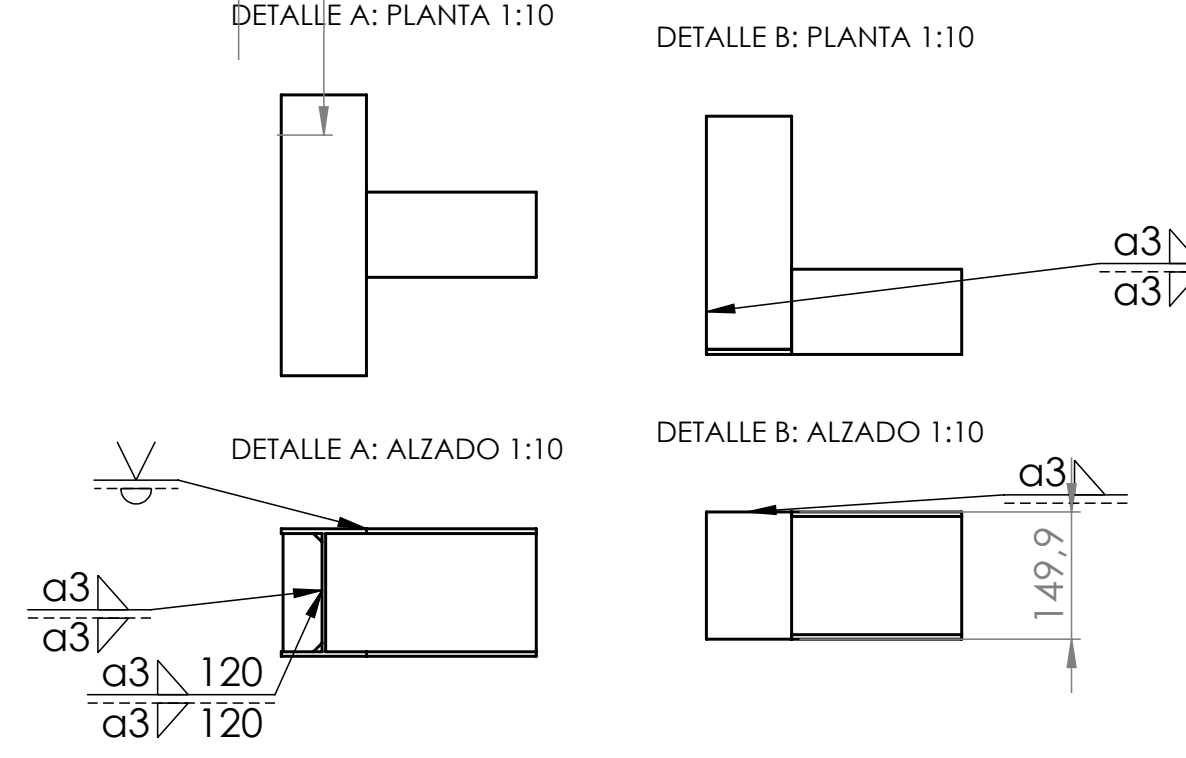
\includegraphics[width=0.80\textwidth]{plano_detalles_uniones.png}
\caption{Detalles del nudo en T (A) y de la esquina (B) del plano del bastidor, con los símbolos de soldadura ISO 2553 \cite{iso2553}. El plano completo está en el Anexo~\ref{anx:planos}. Elaboración propia en SolidWorks.}
\label{fig:plano-uniones}
\end{figure}

El desvío lateral de las ruedas gobierna el bastidor: lleva las vigas longitudinales a 0,82, frente al máximo de 0,28 del modelo con solo cargas verticales, y a 0,89 si el alabeo quedara libre en los nudos. La carga es una envolvente conservadora, porque pone toda la fuerza lateral en una sola rueda. Se descartó omitir los rigidizadores, porque sin ellos no se asegura la continuidad de las alas. Los filetes o cubrejuntas en las alas no caben con alas coplanares y elevarían el ala bajo los apoyos. La fatiga no se evaluó: se estiman unos 2000 ciclos en 20 años, por debajo del umbral de 20\,000 ciclos del apéndice 3 de AISC 360-16 \cite{aisc360}.

\subsubsection{Ruedas, rieles y guiado}
\label{sec:ruedas-rieles}

Con la masa de diseño de 3500 kg (34,3 kN) y una excentricidad del centro de gravedad de $\pm100$ mm, la envolvente de tres contactos con reacciones no negativas alcanzó 19,01 kN por rueda sin factor. La Tabla~\ref{tab:ruedas-rieles} contrasta las demandas con la rueda y el riel seleccionados en la Sección~\ref{sec:seleccion-traslado-rueda}.

\begingroup
\small\singlespacing
\setlength{\parskip}{0pt}
\setlength{\tabcolsep}{4pt}
\renewcommand{\arraystretch}{1.1}
\begin{longtable}{@{}>{\raggedright\arraybackslash}p{4.8cm}>{\raggedright\arraybackslash}p{2.8cm}>{\raggedright\arraybackslash}p{\dimexpr\textwidth-4.8cm-2.8cm-4\tabcolsep\relax}@{}}
\caption{Demandas de rueda y riel frente a los componentes seleccionados}\label{tab:ruedas-rieles}\\
\toprule
\textbf{Magnitud} & \textbf{Valor} & \textbf{Referencia y lectura}\\
\midrule\endfirsthead
\caption[]{Demandas de rueda y riel frente a los componentes seleccionados (continuación)}\\
\toprule
\textbf{Magnitud} & \textbf{Valor} & \textbf{Referencia y lectura}\\
\midrule\endhead
\midrule\multicolumn{3}{r}{\textit{Continúa en la página siguiente.}}\\\endfoot
\bottomrule\endlastfoot
Carga de rueda en servicio ($\times1{,}15$) & 21,87 kN & Capacidad de rodadura de la rueda de 200 mm: 24,52 kN \cite{blickle2026}; D/C 0,89.\\
Carga de rueda resistente ($\times1{,}40$) & 26,62 kN & Capacidad estática: 61,29 kN \cite{blickle2026}; D/C 0,43.\\
Fuerza lateral de guiado por rueda & 6,51 kN & Desvío según EN 1991-3, con $f=0{,}281$ \cite{en19913}.\\
Riel A45 sobre 12 apoyos por riel, paso máximo de 580 mm & 97,9 / 63,7 MPa & Esfuerzos resistentes en cabeza y base; flecha de 0,26 mm en servicio \cite{arcelor2023}.\\
Reacción mínima en un apoyo del riel & $-3{,}78$ kN & Levantamiento: los pedestales se anclan a la losa (Anexo~\ref{anx:calculos}).\\
\end{longtable}
\endgroup

La fuerza lateral de guiado se calculó con la expresión $H_T=f\,Q_r$ del Capítulo~\ref{cap:marco-teorico}, con el desvío y los valores mínimos que fija la norma para el guiado por pestaña \cite{en19913}. Reemplazó al valor de cribado de 7,99 kN usado antes. Con ella, la mejilla de 12 mm de la horquilla dio D/C 0,90, el cordón de la mejilla con la placa dio 0,43 y el eje de la rueda pasó de 140 a 218 MPa (D/C 0,71). Las cuatro ruedas tienen retención axial: el eje lleva cabeza y rosca M33$\times$2 y aprieta las mejillas, los distanciadores y los aros interiores de los rodamientos de la rueda. Los pedestales del riel, que reciben el levantamiento, la fuerza lateral y el tensor de las cadenas, se resumen en el Anexo~\ref{anx:calculos}.

\subsubsection{Traslado de la mesa}
\label{sec:dimensionamiento-traslado}

La fuerza de traslado se calculó con la Ecuación~\eqref{eq:teo-rodadura} para tres escenarios de resistencia de rodadura, con la masa de diseño. Para arrancar se necesitan 120,2 N con el riel nivelado, 324,7 N en el escenario limpio de diseño y 836,7 N en el adverso, con el riel mojado o desalineado; en marcha, 85,8, 256,0 y 665,0 N. Estas fuerzas descartaron el empuje directo (Sección~\ref{sec:seleccion-traslado-rueda}). El sistema seleccionado usa dos cadenas de rodillos 08B de acero inoxidable bajo la mesa, en $X=\pm600$ mm, con un eje motriz de 25 mm y un volante de 400 mm con reductor sinfín de relación 5 fuera de la cabina. Son dos cadenas porque una sola, descentrada 600 mm, tiraría de un lado y sobrecargaría la pestaña de las ruedas. La Tabla~\ref{tab:traslado-verificacion} reúne la verificación.

\begin{table}[htbp]
\centering\small\singlespacing
\caption{Verificación del traslado por doble cadena con volante}
\label{tab:traslado-verificacion}
\begin{tabularx}{\textwidth}{@{}Yrr@{}}
\toprule
\textbf{Elemento y caso} & \textbf{Valor} & \textbf{D/C o margen}\\
\midrule
Fuerza en la empuñadura, arranque de diseño / adverso & 15,5 / 39,8 N & --\\
Cadena, tiro de diseño por cadena (0,5 kN) & -- & FS 21,4\\
Cadena, tiro limitado por el pasador fusible (1,95 kN) & -- & FS 5,5\\
Eje motriz de 25 mm, a 3 kN (sección plena / neta en el chavetero) & 92 / 156 MPa & 0,45 / 0,76\\
Chaveta del piñón, $8\times7$, presión lateral & 93 MPa & 0,51\\
Barra de tiro RHS $60\times40\times4$, a 3 kN & 70 MPa & 0,30\\
Unión de la barra a la viga frontal & -- & 0,10\\
Energía cinética de la mesa: empuje manual / cadena & 39,4 / 1,8 J & --\\
Fuerza de parada en 0,10 m: empuje manual / cadena & 565 / 190 N & --\\
Tiempo de traslado (3,32 m) & 104 s & --\\
\bottomrule
\end{tabularx}
\par\smallskip\footnotesize
La resistencia de la cadena inoxidable se tomó como el 60\,\% de la de acero al carbono; en catálogo, la 08B-1 inoxidable rompe a 12,5 kN frente a unos 18 kN, cerca del 70\,\% \cite{iwis08b}. La sección neta en el chavetero es una cota superior.
\end{table}

La cadena impone la velocidad de la mesa, de 0,032 m/s. Con ella, la energía cinética baja de 39,4 a 1,8 J y la fuerza para detener la mesa en 0,10 m, de 565 a 190 N, por lo que no se requiere un freno aparte. Un pasador fusible de latón en el volante limita el tiro total a 3 kN y protege la cadena ante un mal uso; en las estaciones, la retención sigue a cargo del pasador de bloqueo. El eje motriz se redujo de 30 a 25 mm porque la revisión de interferencias encontró que el cubo del piñón chocaba con la cadena.
 El reductor admite un motor con brida; la motorización del traslado queda como recomendación (Capítulo~\ref{cap:conclusiones}).

\subsubsection{Centradores}
\label{sec:dimensionamiento-centradores}

Los centradores posicionan el rodamiento sin soportar su peso. Se dispusieron tres unidades con brazo pivotante de eje vertical alrededor del diámetro exterior: dos actúan como referencias rígidas (sobre los travesaños de carga) y la tercera, el centrador empujador sobre una viga longitudinal, lleva el aro contra ellas con fuerza normal limitada. El empujador se detiene cuando la normal en su rodillo alcanza 1,45 kN, con un disparo independiente a 1,60 kN; el límite de ensayo es de 2,08 kN. El brazo del empujador mide 67,15 mm y el contacto se produce a $Z=955$ mm.

El soporte de cada referencia se dimensionó con un modelo de elementos finitos de sólidos del tramo de perfil, la mordaza y las placas, bajo 2,08 kN, con dos niveles de malla y los dos sentidos de carga. Las referencias dieron un desplazamiento radial de 0,48 a 0,59 mm en el punto de contacto, con error de equilibrio no mayor que 0,68\,\%. Las mordazas de las referencias se fijan al alma de los travesaños con dos pernos M12 de clase 8.8 pasantes; la del empujador, con dos pernos pasantes M12 por el alma de la viga longitudinal. La placa del soporte del pivote del empujador se fijó en 28 mm, con soldaduras a tope con penetración completa contra el pedestal. La captura y la precisión del centrado se presentan en la sección siguiente y en la Sección~\ref{sec:resultados-soporte}.

\subsubsection{Error de colocación del rodamiento}
\label{sec:error-colocacion}

El requisito E06 limita a 5 mm el error radial de colocación. La versión anterior del centrado obtuvo 5,21 mm en el caso nominal y 6,10 mm en la envolvente de 2,08 kN, ambos con suma aritmética de tolerancias. Para corregirlo por diseño se separaron las dos partes de la Ecuación~\eqref{eq:mt-colocacion}: el desplazamiento elástico de las referencias, calculado con SAP2000 y con el modelo de barras con alabeo, y la suma de tolerancias de fabricación, juegos, rodillos, diámetro exterior del aro, temperatura y apoyo con la grúa, que vale 1,58 mm. Luego se recalculó el error para cada fuerza que el mecanismo puede dejar en el rodillo (Tabla~\ref{tab:centrado-por-fuerza} y Figura~\ref{fig:centrado}).

\begin{table}[htbp]
\centering\small\singlespacing
\caption{Error de colocación del rodamiento según la fuerza final del centrador empujador}
\label{tab:centrado-por-fuerza}
\begin{tabularx}{\textwidth}{@{}Yrrrr@{}}
\toprule
\textbf{Estado del centrador empujador} & \textbf{Fuerza en} & \multicolumn{3}{c}{\textbf{Error de colocación (mm) según el alabeo}}\\
\cmidrule(l){3-5}
 & \textbf{el rodillo} & \textbf{Libre} & \textbf{Alas continuas} & \textbf{Impedido}\\
\midrule
Detención operativa & 1,45 kN & 4,09 & 3,35 & 3,02\\
Disparo independiente del limitador de fuerza & 1,60 kN & 4,24 & 3,35 & 3,00\\
Límite de ensayo: fallan la detención y el disparo & 2,08 kN & 5,18 & 3,91 & 3,45\\
Fricción asimétrica de 0,30, suma algebraica & $\approx3{,}1$ kN & 5,51 & 5,01 & 4,24\\
\midrule
\textbf{Requisito E06} & & \multicolumn{3}{c}{$\leq5{,}00$}\\
\bottomrule
\end{tabularx}
\par\smallskip\footnotesize
Rigidez reducida (0,8\,EI) y 1,58 mm de tolerancias en suma aritmética. La última fila supone fuerzas por encima del disparo del limitador.
\end{table}

\begin{figure}[htbp]
\centering
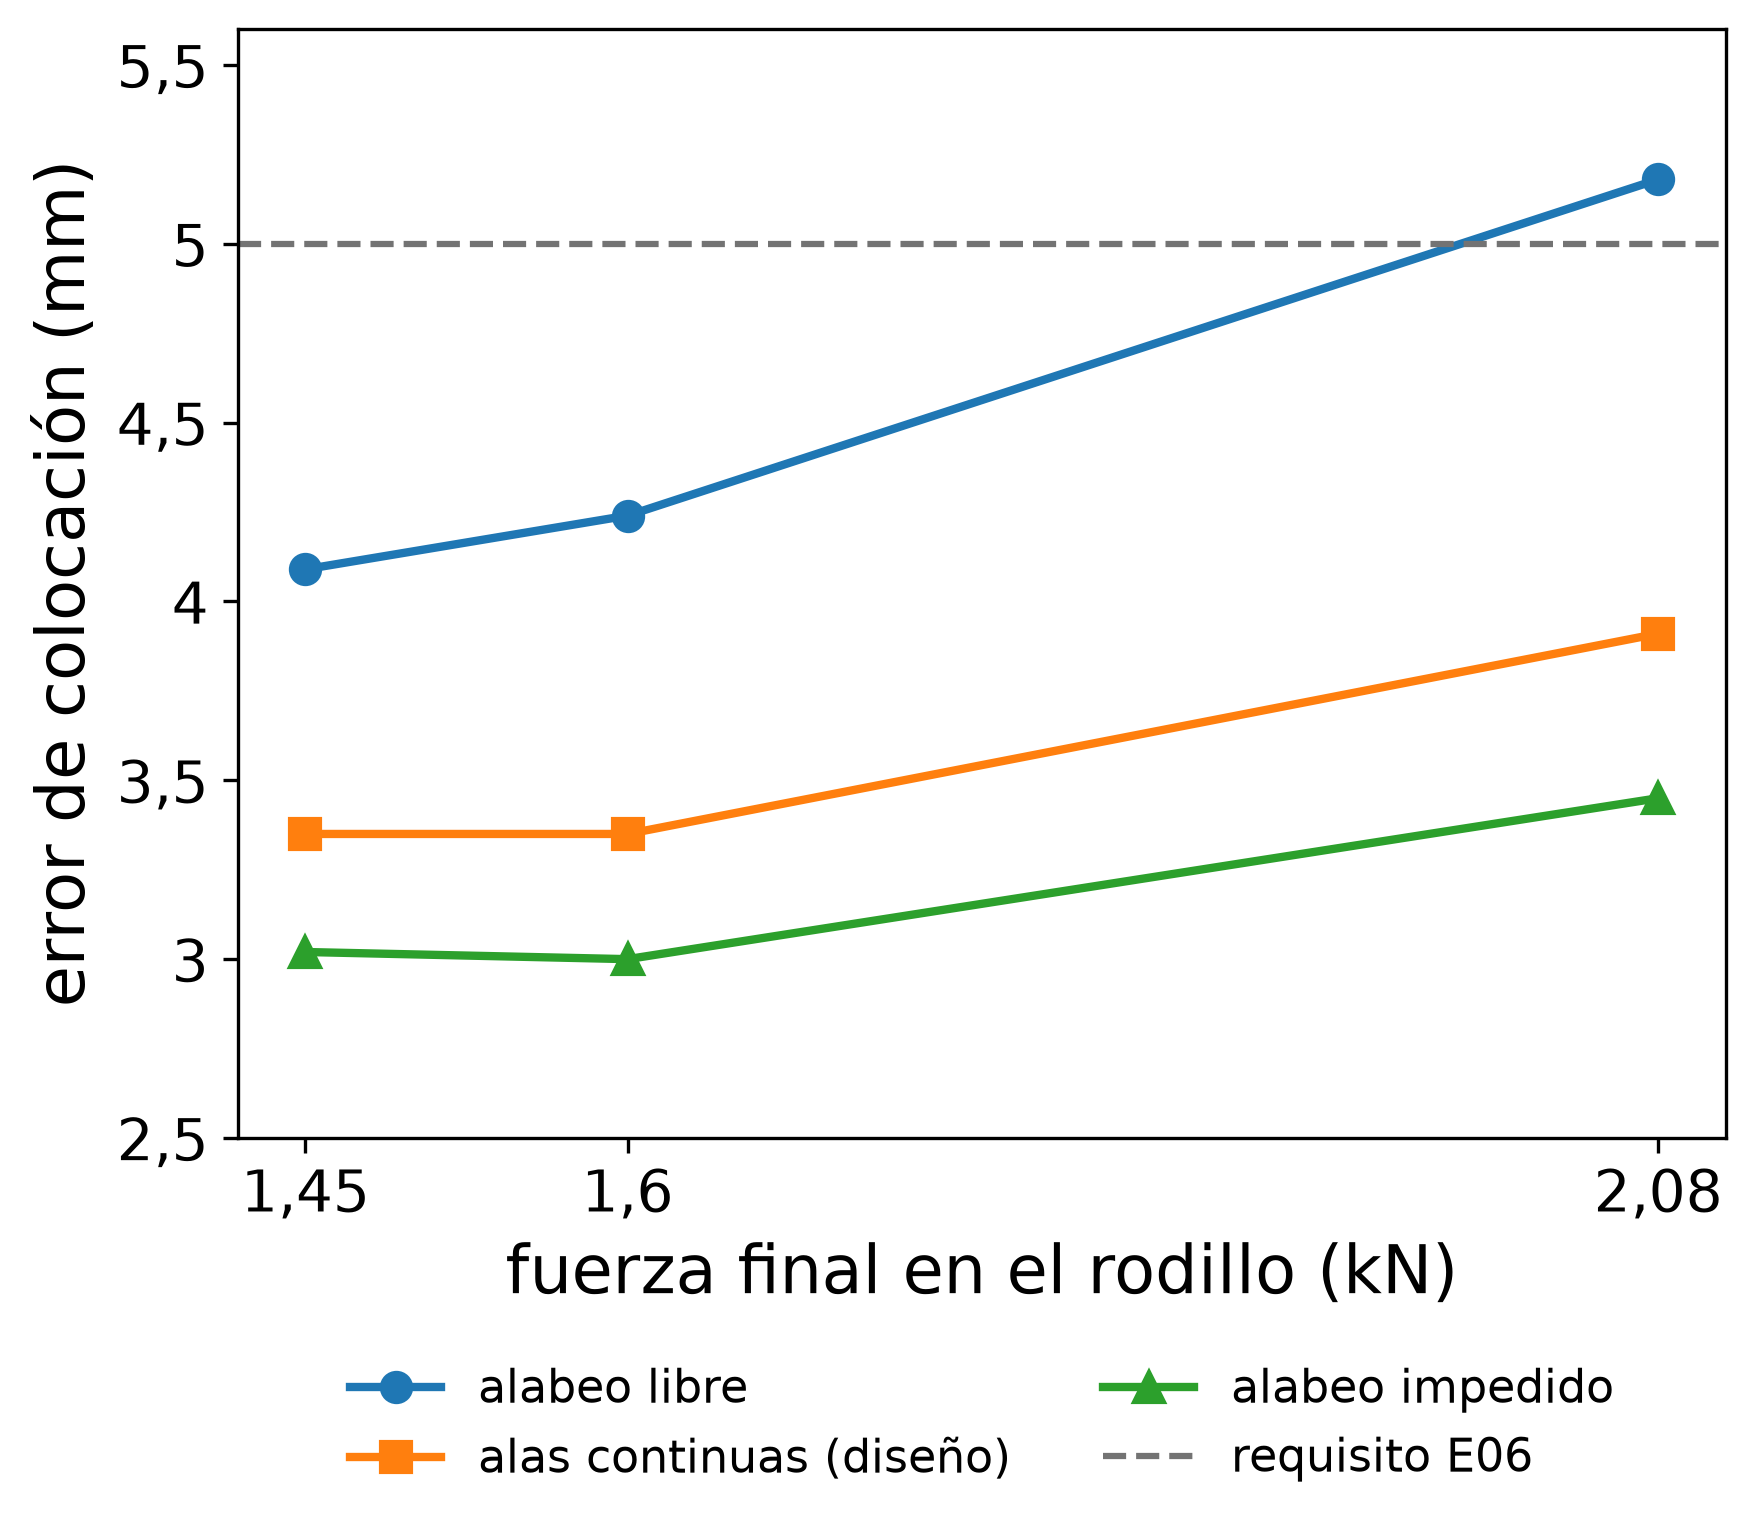
\includegraphics[width=0.62\textwidth]{fig_error_colocacion.png}
\caption{Error de colocación del rodamiento según la fuerza final en el rodillo del centrador empujador y la condición de alabeo en los nudos del bastidor. Elaboración propia con los resultados del modelo de barras.}
\label{fig:centrado}
\end{figure}

El ajuste H7/g6 \cite{iso286} se especificó en el pasador de bloqueo de 25 mm, en los pivotes de los brazos y en los pasadores de los rodillos; con él, todos los juegos suman 0,121 mm. A 2,08 kN, el 70\,\% del error es deformación elástica: 3,60 de 5,18 mm. Esa parte es lineal con la fuerza, con 1,731 mm/kN si el alabeo queda libre, y por eso el requisito se cumple mientras la fuerza final no pase de 1,97 kN. Se fijó entonces un requisito al limitador de fuerza del empujador: la fuerza final en el rodillo no debe pasar de 1,95 kN, incluida la dispersión del disparo. Con las alas continuas que da el detalle de uniones, el error baja a 3,35 mm en operación y a 3,91 mm en la envolvente.

Se evaluó y se descartó un cono de indexado en el pasador. Un cono solo elimina juego: llevaría el error de 5,18 a 5,14 mm, y aun sin ningún juego quedaría en 5,06 mm. Además, el pasador recibe hasta 1184 N en la estación de carga, un cono que no se autobloquea necesita otra pieza que lo mantenga asentado, y su asiento acumula grasa y agua alcalina. Apretar las tolerancias tampoco convenía: obligaría a mecanizar la mesa soldada para ganar apenas 0,05 mm.

\subsubsection{Bloqueo y retención}

La mesa se inmoviliza con el pasador central de 25 mm a doble corte, predimensionado para 10 kN, que se inserta en un receptor de la estación de carga antes de centrar y en otro de la estación de lavado antes de retraer los centradores. Tres topes bajos, a 60$^\circ$, 190$^\circ$ y 300$^\circ$, retienen el aro si este se desplaza sobre los apoyos; su unión al bastidor se detalla en los planos del Anexo~\ref{anx:planos}.

\subsection{Subsistema de aspersión}
\label{sec:dimensionamiento-aspersion}

\subsubsection{Caudal por boquilla y número de boquillas}

Con la Ecuación~\eqref{eq:teo-boquilla} y el punto de catálogo (7,571 L/min a 2,758 bar), el caudal de una boquilla a 4 bar resultó
\begin{equation}
q=q_r\sqrt{\frac{p_n}{p_r}}=7{,}571\sqrt{\frac{4{,}000}{2{,}758}}=9{,}118\ \mathrm{L/min},
\label{eq:dis-q-boquilla}
\end{equation}
con velocidad característica $v_j=C_v\sqrt{2p_n/\rho}=27{,}1$ m/s. Las boquillas de 15$^\circ$ tienen la misma capacidad nominal que las de 50$^\circ$, por lo que el mismo cálculo vale para ambas; solo cambia el abanico. El número de boquillas de cada grupo se obtuvo con la huella del abanico (Ecuación~\eqref{eq:teo-huella}) y la condición de solape:
\begin{equation}
N\geq1+\frac{L-b}{b(1-\phi)}.
\label{eq:dis-numero-boquillas}
\end{equation}
Para la lanza, con $L=515$ mm, distancia de 143,3 mm y $b=2(143{,}3)\tan25^\circ=133{,}6$ mm, resultó $N\geq4{,}81$; se adoptaron cinco boquillas, con un solape nominal de 28,7\,\%. Los grupos superior y exterior se dimensionaron del mismo modo. La Tabla~\ref{tab:boquillas-grupos} compara las tres configuraciones que se calcularon.

\begin{table}[htbp]
\centering\small\singlespacing
\caption{Distribución de boquillas del caso analítico, de la configuración base y de la configuración propuesta}
\label{tab:boquillas-grupos}
\begin{tabular}{@{}lccc@{}}
\toprule
\textbf{Grupo} & \textbf{Caso analítico} & \textbf{Base} & \textbf{Propuesta}\\
\midrule
Laterales exteriores ($2$ brazos) & $2\times5$ & $2\times5$ & $2\times5$\\
Superiores ($2$ brazos) & $2\times2$ & $2\times2$ & $2\times2$\\
Lanza interior (agujero) & 5 & 5 & 5\\
Inferior interior (lanza) & --- & 1 & 1\\
Inferiores exteriores (2 brazos) & --- & $2\times1$ & $2\times2$\\
\midrule
\textbf{Total simultáneo} & \textbf{19} & \textbf{22} & \textbf{24}\\
\bottomrule
\end{tabular}
\end{table}

\subsubsection{Configuración inferior}
\label{sec:configuracion-inferior}

La simulación de la configuración base mostró que la cara inferior recibía unas cuatro veces menos dosis que las demás superficies (Sección~\ref{sec:resultados-aspersion}). La causa era geométrica. La boquilla inferior exterior salía unos 35 a 40 mm bajo la cara, inclinada 30$^\circ$, y su eje llegaba al radio de 710 mm a una altura de unos 928 mm: mojaba la parte baja del diámetro exterior y no la cara inferior. Agregar caudal sin cambiar la geometría no resolvía la zona exterior de la cara.

Se compararon alternativas con trazado de rayos y se eligió un par de boquillas de abanico estrecho (15$^\circ$) en cada brazo. La boquilla inferior existente se reorientó a 15$^\circ$, de modo que llega a la cara en el radio de unos 687 mm, y se agregó otra a 10,7$^\circ$, que llega en el radio de unos 624 mm, separadas 60 mm. Las dos van en un bloque portaboquillas mecanizado de acero inoxidable. La red pasa de 22 a 24 boquillas: 20 de 50$^\circ$ y 4 de 15$^\circ$. Además, la primera boquilla lateral de cada brazo se inclinó 4$^\circ$ hacia abajo, con su punta fija, para cerrar una franja seca de 2 mm del diámetro exterior. El efecto de estos cambios en el mojado se evaluó con CFD y se analiza en la Sección~\ref{sec:resultados-aspersion}.

Para fijar las tolerancias de soldadura de las coplas, se perturbó cada boquilla con trazado de rayos en 240 casos de $\pm2$ mm y $\pm1^\circ$. Las coplas de 50$^\circ$ cambiaron la dosis como máximo un 2,8\,\%. Las salidas de 15$^\circ$ del bloque inferior, que llegan casi rasantes, perdían hasta un 18\,\%; por eso al bloque mecanizado se le asignaron $\pm0{,}5^\circ$ y $\pm1$ mm, con pérdidas de hasta 9,4\,\%. El criterio de 10\,\% es una hipótesis de los autores, y el trazado de rayos es un cribado del primer impacto, no un CFD.

\subsubsection{Red hidráulica, altura de bombeo y potencia}

La red se resolvió por aproximaciones sucesivas: con la Ecuación~\eqref{eq:teo-perdidas} y el factor de fricción de Swamee--Jain \cite{manSwamee}, se calcularon las pérdidas de cada tramo y se ajustó la presión de alimentación hasta que la boquilla más desfavorable recibiera 4 bar. La altura de bombeo se obtuvo con la Ecuación~\eqref{eq:teo-energia} entre la superficie libre del depósito y el cubo distribuidor, y la potencia con la Ecuación~\eqref{eq:teo-potencia}. El guion de cálculo reprodujo primero el caso analítico de diecinueve boquillas con las mismas cifras. La Tabla~\ref{tab:red-hidraulica} da los resultados de las tres configuraciones.

\begin{table}[htbp]
\centering\small\singlespacing
\caption{Resultados de la red hidráulica por configuración}
\label{tab:red-hidraulica}
\begin{tabularx}{\textwidth}{@{}Yccc@{}}
\toprule
\textbf{Magnitud} & \textbf{19 boquillas} & \textbf{22 boquillas} & \textbf{24 boquillas}\\
\midrule
Caudal total (L/min) & 173,99 & 202,59 & 221,07\\
Boquilla más desfavorable & Superior & Lanza & Lanza\\
Presión en las boquillas (bar) & 4,00--4,06 & 4,00--4,14 & 4,00--4,13\\
Altura de bombeo (m) & 50,75 & 52,56 & 53,39\\
Velocidad en DN40 (m/s) & 2,02 & 2,35 & 2,57\\
Potencia hidráulica (kW) & 1,42 & 1,71 & 1,90\\
Potencia al eje, $\eta_p=0{,}55$ (kW) & 2,58 & 3,11 & 3,45\\
\bottomrule
\end{tabularx}
\par\smallskip\footnotesize
Las tres columnas suponen una alimentación de 14 m en DN40. Con el trazado del modelo integrado, la altura de la red de 24 boquillas baja a 50,98--51,29 m.
\end{table}

Con 24 boquillas, el caudal sube un 9,1\,\% y la altura un 0,83 m respecto de la red de 22. La boquilla más alta de la lanza sigue fijando la presión del cubo en 4,063 bar, y las boquillas existentes cambian su presión en menos de 10 mbar, es decir, menos del 0,12\,\% en caudal. Por eso las superficies que no cambiaron de boquillas conservan los resultados de la simulación anterior.

Las alturas de la tabla suponen 14 m de alimentación en DN40 a 2,57 m/s. El modelo integrado tiene, en cambio, 8,7 m de tubería DN50 a 1,56 m/s hasta la unión rotativa; con ese trazado, la altura requerida es de 50,98 m con el tanque en su nivel normal y de 51,29 m en el nivel bajo. La subida hasta la unión rotativa no suma altura estática, porque se recupera al bajar hasta el cubo. Se informan las dos cifras: 53,39 m es la cota del cálculo de la red y 51,0--51,3 m, la del trazado modelado.

Se seleccionó una bomba multietapa vertical Grundfos CRN 15-3 de acero inoxidable 316, con motor de 4 kW \cite[pp.~50--51]{grundfoscr}. En la curva del catálogo entrega unos 56 m a 13,3 m$^3$/h, con unos 3,0 kW en el eje y un rendimiento cercano al 65\,\%; son lecturas gráficas, con una incertidumbre de $\pm1$ m en la altura. Le sobran de 2,6 a 4,7 m según la altura que se tome; ese exceso se recorta con un variador de frecuencia ajustado para que la boquilla más desfavorable reciba 4,00 bar. El NPSH disponible, con la presión atmosférica de 2335 m y la presión de vapor a 62~$^\circ$C, es de 5,24 a 5,55 m según el nivel del tanque \cite{white2016}, frente a unos 2,2 m requeridos por la bomba, valor conservador respecto de su curva. La potencia al eje de la Tabla~\ref{tab:red-hidraulica} usa un rendimiento supuesto de 0,55; con el de catálogo, la demanda es menor. La memoria de la red está en el Anexo~\ref{anx:calculos}.

\subsubsection{Distribuidor giratorio, eje y cubo}
\label{sec:distribuidor}

El distribuidor en U gira sobre un eje hueco, por cuyo interior pasa la alimentación hasta un cubo que reparte el caudal a la U y a la lanza (planos del eje, del cubo y de la U en el Anexo~\ref{anx:planos}). Para verificarlo se tomó la masa del modelo CAD, con 148 sólidos y el agua en los tubos. La estimación anterior era una envolvente de 180 kg con 50 mm de excentricidad; el modelo dio 231 kg con el centro de gravedad a 79,6 mm del eje, de modo que el momento excéntrico pasó de 88 a 180 N\,m. Como esa excentricidad gira con el eje, el peso produce una tensión constante en el eje; la única flexión alterna es la de la correa, que tira siempre en la misma dirección.

Las cargas fueron el peso y la excentricidad medidos, un par de 60 N\,m (el limitador desliza), un tiro de correa de 1071 N, la reacción de los chorros de 97 N, una carga accidental de 1000 N horizontal a 1400 mm del piso y una presión de 6 bar, con prueba hidrostática a 9 bar. Los 1071 N son una envolvente conservadora del tiro de la correa: el motorreductor se verificó con los 625 N que resultan del par limitado. La carga accidental y la presión son hipótesis de diseño. La Tabla~\ref{tab:conjunto-giratorio} reúne la verificación.

\begin{table}[htbp]
\centering\small\singlespacing
\caption{Verificación del distribuidor giratorio, su eje y su cubo}
\label{tab:conjunto-giratorio}
\begin{tabularx}{\textwidth}{@{}Yllr@{}}
\toprule
\textbf{Elemento y caso} & \textbf{Método} & \textbf{Resultado} & \textbf{D/C}\\
\midrule
Eje en el asiento del rodamiento inferior, accidental & von Mises & 37,4 MPa & 0,27\\
Eje en la polea, con chavetero, accidental & von Mises & 15,6 MPa & 0,11\\
Fatiga del eje en la polea & Goodman, Ec.~\eqref{eq:mt-goodman} & $\sigma_a=\sigma_m=4{,}9$ MPa & $n_f=24$\\
Flecha en las boquillas, servicio & Viga con voladizo & 0,36 mm y 0,31 mrad & --\\
Tubería junto al cubo, cargas sostenidas & ASME B31.3 \cite{asmeb313} & 13,4 MPa & 0,13\\
Codo de reducción, carga ocasional & ASME B31.3 & 100,5 MPa & 0,74\\
Tubería junto al cubo, carga ocasional tangencial & ASME B31.3 & 126,4 MPa & 0,93\\
Placas del cubo a 6 bar, borde empotrado & Placa circular & 60,6 MPa & 0,59\\
Placas del cubo en la prueba a 9 bar & Placa circular & 91 MPa & 0,66\\
Unión del eje con el cubo, filete de 5 mm & Cordón circular & 17,3 MPa & 0,05\\
\bottomrule
\end{tabularx}
\par\smallskip\footnotesize
Acero inoxidable 316L con $f_y=170$ MPa, reducido a 153 MPa a 62~$^\circ$C (hipótesis).
\end{table}

La resistencia no fija el tamaño del eje: lo fijan el paso de la alimentación por dentro y los asientos de 110 mm. La flecha de servicio en las boquillas es el 18\,\% de la tolerancia supuesta para el CFD. El único valor alto de la U, 0,93, corresponde a la carga accidental tangencial en un brazo, que solo puede ocurrir con el rotor detenido; con el rotor libre, el limitador desliza con 67 N en la punta del brazo. Las verificaciones complementarias con sólidos (Anexo~\ref{anx:calculos}) muestran que ese mismo golpe de 1000 N produce fluencia local en el tubo junto a la soldadura del transversal con el cubo, mientras la sección general trabaja al 74\,\% de la fluencia. Con el tramo central del transversal en DN50 Sch 80S, de igual diámetro exterior, la misma simulación deja la unión bajo la fluencia, con un margen de 1,23, sin cambiar las bridas ni el cordón; se recomienda esa variante. Las placas de 15 mm del cubo cumplen solo si se sueldan al anillo con penetración completa: el anillo es 15,5 veces más rígido al giro que la placa, lo que justifica tomar el borde como empotrado. Con borde apoyado, la prueba a 9 bar daría 1,09; por eso el requisito quedó escrito en el plano del eje y el cubo.

El cubo se suelda al eje y ambos se mecanizan en una sola atada, de modo que los asientos de los rodamientos y la cara inferior del cubo quedan alineados. La alternativa bridada con espiga H7/g6 sumaba una brida, seis pernos, una junta tórica expuesta al detergente a 62~$^\circ$C y unos 5 kg, sin una ventaja de resistencia: las dos uniones dan D/C $\leq0{,}06$. La U se desmonta por dos juntas bridadas DN50 a 300 mm del eje, sin válvulas de ramal, y sus dos brazos son iguales; en cada junta, el perno más cargado lleva 1,16 kN frente a 70,7 kN (D/C 0,02). Ninguna boquilla cambió de posición, de modo que el CFD sigue siendo válido para esta geometría.

El distribuidor gira con un motorreductor de 0,12 kW a través de una correa con relación 2:1. El limitador de par va en el eje de salida del motorreductor, ajustado a 30 N\,m, que equivalen a 60 N\,m en el rotor. Sin limitador, un atasco llevaría la carga radial de ese eje a 3,9 kN y no pasaría; con él, la carga radial es de 625 N según el método del fabricante y el factor de seguridad, de 2,31. El soporte superior que sostiene el conjunto y la selección del accionamiento se resumen en el Anexo~\ref{anx:calculos}.

\subsubsection{Cinemática del distribuidor}

A 1,7 rpm, una vuelta del distribuidor dura 35,3 s. La velocidad de barrido de las boquillas exteriores, a un radio de 836 mm, es de 0,149 m/s, y la de la lanza, 0,055 m/s. El tiempo de vuelo de las gotas hasta la superficie, de unos 7 ms a la mayor distancia, es pequeño frente al período de giro, lo que justifica evaluar la dosis con el distribuidor detenido por sectores (Sección~\ref{sec:teo-cfd}).

\subsubsection{Temperatura del baño}
\label{sec:calentamiento}

El detergente seleccionado no forma espuma por encima de 61~$^\circ$C y admite hasta 70~$^\circ$C \cite{zep36342}, por lo que el lavado se plantea con el baño a 60--62~$^\circ$C. Las lavadoras comerciales de aspersión calientan el tanque con resistencias de inmersión o con un quemador a gas, ofrecen un intercambiador de calor como opción y regulan la temperatura con un control electrónico: el StingRay 6075, con un depósito de 1325 L, usa 60 kW eléctricos o 117 kW a gas y tarda de 45 a 120 min en calentar el baño \cite{stingray_6075}. La máquina necesita un sistema equivalente. El esquema hidráulico lo representa con resistencias de inmersión y un control de temperatura en el tanque de lavado, como referencia de integración; su selección y su dimensionamiento quedan fuera del alcance.
